% Choose one to switch between slides and handout
%\documentclass[]{beamer}
\documentclass[handout]{beamer}

% Video Meta Data
\title{Smart Contracts and Decentralized Finance}
\subtitle{Lending Protocols}
\author{Prof. Dr. Fabian Schär}
\institute{University of Basel}

% Config File
% Packages
\usepackage[utf8]{inputenc}
\usepackage{hyperref}
\usepackage{gitinfo2}
\usepackage{tikz}
 \usetikzlibrary{calc}
\usepackage{amsmath}
\usepackage{mathtools}
\usepackage{bibentry}
\usepackage{xcolor}
\usepackage{colortbl} % Add colour to LaTeX tables
\usepackage{caption}
\usepackage[export]{adjustbox}
\usepackage{pgfplots} \pgfplotsset{compat = 1.17}
\usepackage{makecell}
\usepackage{fancybox}
\usepackage{ragged2e}
\usepackage{fontawesome}
\usepackage{seqsplit}
\usepackage{tabularx}
\usepackage{tcolorbox}
\usepackage{booktabs} % use instead  \hline in tables

% Color Options
\definecolor{highlight}{rgb}{0.65,0.84,0.82}
\definecolor{focus}{rgb}{0.72, 0, 0}
\definecolor{lightred}{rgb}{0.8,0.5,0.5}
\definecolor{midgray}{RGB}{190,195,200}

 %UniBas Main Colors
\definecolor{mint}{RGB}{165,215,210}
\definecolor{anthracite}{RGB}{45,55,60}
\definecolor{red}{RGB}{210,5,55}

 %UniBas Color Palette (for graphics)
\definecolor{strongmint}{RGB}{30,165,165}
\definecolor{darkmint}{RGB}{0,110,110}
\definecolor{softanthracite}{RGB}{140,145,150}
\definecolor{brightanthracite}{RGB}{190,195,200}
\definecolor{softred}{RGB}{235,130,155}

%Custom Colors
\definecolor{lightergray}{RGB}{230, 230, 230}



% Beamer Template Options
\beamertemplatenavigationsymbolsempty
\setbeamertemplate{footline}[frame number]
\setbeamercolor{structure}{fg=black}
\setbeamercolor{footline}{fg=black}
\setbeamercolor{title}{fg=black}
\setbeamercolor{frametitle}{fg=black}
\setbeamercolor{item}{fg=black}
\setbeamercolor{}{fg=black}
\setbeamercolor{bibliography item}{fg=black}
\setbeamercolor*{bibliography entry title}{fg=black}
\setbeamercolor{alerted text}{fg=focus}
\setbeamertemplate{items}[square]
\setbeamertemplate{enumerate items}[default]
\captionsetup[figure]{labelfont={color=black},font={color=black}}
\captionsetup[table]{labelfont={color=black},font={color=black}}

\setbeamertemplate{bibliography item}{\insertbiblabel}

%tcolor boxes
\newtcolorbox{samplecode}[2][]{
  colback=mint, colframe=darkmint, coltitle=white,
  fontupper = \ttfamily\scriptsize, fonttitle= \bfseries\scriptsize,
  boxrule = 0mm, arc = 0mm,
  boxsep = 1.3mm, left = 0mm, right = 0mm, top = 0.5mm, bottom = 0mm, middle=0mm,
  #1,title=#2}
  
\newtcolorbox{keytakeaway}[2][]{
  colback=softred, colframe=red, coltitle=white,
  fontupper = \scriptsize, fonttitle= \bfseries\scriptsize,
  boxrule = 0mm, arc = 0mm,
  boxsep = 1.3mm, left = 0mm, right = 0mm, top = 0.5mm, bottom = 0mm, middle=0mm,
  #1,title=#2}

\newtcolorbox{exercise}[2][]{
  colback=brightanthracite, colframe=anthracite, coltitle=white,
  fontupper = \scriptsize, fonttitle= \bfseries\scriptsize,
  boxrule = 0mm, arc = 0mm,
  boxsep = 1.3mm, left = 0mm, right = 0mm, top = 0.5mm, bottom = 0mm, middle=0mm,
  #1,title=#2}



% Link Icon Command 
\newcommand{\link}{%
    \tikz[x=1.2ex, y=1.2ex, baseline=-0.05ex]{%
        \begin{scope}[x=1ex, y=1ex]
            \clip (-0.1,-0.1)
                --++ (-0, 1.2)
                --++ (0.6, 0)
                --++ (0, -0.6)
                --++ (0.6, 0)
                --++ (0, -1);
            \path[draw,
                line width = 0.5,
                rounded corners=0.5]
                (0,0) rectangle (1,1);
        \end{scope}
        \path[draw, line width = 0.5] (0.5, 0.5)
            -- (1, 1);
        \path[draw, line width = 0.5] (0.6, 1)
            -- (1, 1) -- (1, 0.6);
        }
    }

% Other commands
\newcommand\tab[1][0.5cm]{\hspace*{#1}} % for code boxes


% Read Git Data from Github Actions Workflow
% Defaults to gitinfo2 for local builds
\IfFileExists{gitInfo.txt}
	{\input{gitInfo.txt}}
	{
		\newcommand{\gitRelease}{(Local Release)}
		\newcommand{\gitSHA}{\gitHash}
		\newcommand{\gitDate}{\gitAuthorIsoDate}
	}

% Custom Titlepage
\defbeamertemplate*{title page}{customized}[1][]
{
  \vspace{-0cm}\hfill\includegraphics[width=2.5cm]{../config/logo_cif}
  \includegraphics[width=1.9cm]{../config/seal_wwz}
  \\ \vspace{2em}
  \usebeamerfont{title}\textbf{\inserttitle}\par
  \usebeamerfont{title}\usebeamercolor[fg]{title}\insertsubtitle\par  \vspace{1.5em}
  \small\usebeamerfont{author}\insertauthor\par
  \usebeamerfont{author}\insertinstitute\par \vspace{2em}
  \usebeamercolor[fg]{titlegraphic}\inserttitlegraphic
    \tiny \noindent \texttt{Release Ver.: \gitRelease}\\ 
    \texttt{Version Hash: \gitSHA}\\
    \texttt{Version Date: \gitDate}\\ \vspace{1em}
    
    
    \iffalse
  \link \href{https://github.com/cifunibas/Bitcoin-Blockchain-Cryptoassets/blob/main/slides/intro.pdf}
  {Get most recent version}\\
  \link \href{https://github.com/cifunibas/Bitcoin-Blockchain-Cryptoassets/blob/main/slides/intro.pdf}
  {Watch video lecture}\\ 
  
  \fi
  
  \vspace{1em}
  License: \texttt{Creative Commons Attribution-NonCommercial-ShareAlike 4.0 International}\\\vspace{2em}
  \includegraphics[width = 1.2cm]{../config/license}
}


% tikzlibraries
\usetikzlibrary{decorations.pathreplacing}
\usetikzlibrary{decorations.markings}
\usetikzlibrary{positioning}
\usetikzlibrary{calc}
\captionsetup{font=footnotesize}

%%%%%%%%%%%%%%%%%%%%%%%%%%%%%%%%%%%%%%%%%%%%%%
%%%%%%%%%%%%%%%%%%%%%%%%%%%%%%%%%%%%%%%%%%%%%%
\begin{document}

\thispagestyle{empty}
\begin{frame}[noframenumbering]
	\titlepage
\end{frame}

%%%
\begin{frame}{Introduction}
Besides exchanging assets, \textbf{borrowing} and \textbf{lending} are the most fundamental needs in a financial system. \\

\vspace{1em}
Due to openness and pseudonymity, DeFi loans exist in two formats:
\vspace{0.5em}
\begin{enumerate}
  \item \textbf{Collaterallized loans} of undefined duration.
  \item \textbf{Flash loans} that are borrowed and repaid in one transaction. 
\end{enumerate} 

\vspace{1em}
Currently, we can distinguish two main lending protocol archetypes in DeFi: \textbf{Collateral Debt Protocols} and \textbf{Collateral Debt Markets}.
	
\end{frame}
%%%	


%%%
\begin{frame}{Some Terminology around Lending in DeFi}

\vspace{1em}

\textbf{Position}: Entirety of an address' collateral $c$ and debt $d$ with a protocol.
			
\vspace{1.0em}
			
\uncover<2-> {
\textbf{Loan-to-Value} (\textit{LTV}): Percentage at which the value of a collateral asset counts towards borrowing capacity. $LTV_i \in [0,1]$
}

\vspace{1.0em}

\uncover<3->{ 
\textbf{Borrowing capacity} (BC): Total amount a position may borrow, given the value of its collateral assets and their respective $LTV$.

\begin{equation}
	BC = \sum c_i\, LTV_i 
	\label{eq:BC} 
\end{equation}
}

\uncover<4->{ 
$\rightarrow$ A position can only take up new debt as long as its existing  debt across all assets is below borrowing capacity, i.e., $BC > \sum d_i$
}

\end{frame}
%%%	


%%%
\begin{frame}{Some Terminology around Lending in DeFi}

\vspace{1em}

\textbf{Liquidation Threshold} (LT): Threshold of debt relative to collateral at which a position becomes unhealthy and thus can be liquidated. $LT_i \in [0,1]$ and $LT_i \geq LTV_i$.

	\begin{equation}
	  		LT =  \frac{\sum c_i \, LT_i}{\sum c_i}
	  	\label{eq:LT} 
	\end{equation}
	

\vspace{1.0em}
\uncover<2->{
\textbf{Health Factor} (HF): Relative value of collateral, adjusted by LT, to outstanding debt of a position.

\begin{equation}
	  HF = \frac{\sum c_i \, LT_i}{\sum d_i} \label{eq:HF} 
\end{equation}

\vspace{1.0em}
$\rightarrow$ A position with $HF \geq 1$ it is considered \color{focus} \textit{healthy} \color{black} .

$\rightarrow$ Collateral of \color{focus} \textit{unhealthy}\color{black} positions is available for liquidation.
}

\end{frame}
%%%





%%%
\begin{frame}{Collateral Debt Protocols (CDP)}

\vspace{-1em}

\begin{figure}[t]
	\centering
	\begin{tikzpicture}[scale=1.0, every node/.style={scale=1.0}]
		
% Figures

\node (borrower) at (-8,0) {\includegraphics[height = 1.7cm]{../assets/images/agents/handing_right}};
\node [below of = borrower, yshift = -0.4cm] {\textbf{Alice}};

\node (protocol) at (0,0) {\includegraphics[height = 1.7cm]{../assets/images/smart_contract}};
\node [below of = protocol, yshift = -0.4cm] {\textbf{CDP}};

% Arrows with text

\footnotesize

\uncover<2->{
\draw[->, black]	([yshift=0.2cm]borrower.east) -- ([yshift=0.2cm]protocol.west) node[midway, fill=white, text = darkmint, align = center] {\textbf{Asset $X$}};
}

\uncover<3->{
\draw[<-, black]	([yshift=-0.2cm]borrower.east) -- ([yshift=-0.2cm]protocol.west) node[midway, fill=white, text = darkmint, align = center] {\textbf{Loan in newly minted $Y$}};
}

	\end{tikzpicture}
\end{figure}

\small
\vspace{-1em}
\begin{columns}[T]
	\begin{column}{0.49\textwidth}
	\uncover<2->{
		\begin{itemize}
			\item	Stays invested in assets provided as collateral.
			\item	Can borrow the CDP issued asset within the borrowing capacity.
			\item	Owes interest for the debt in the CDP asset until repayment.
		\end{itemize}
	}
	\end{column}
	\begin{column}{0.49\textwidth}
	\uncover<3->{
		\begin{itemize}
			\item	Issues a protocol asset and sets borrowing terms.
			\item	Controls the collateral assets as long as there is outstanding debt to cover.
			\item	Allows liquidation of collateral against protocol asset for unhealthy positions.
		\end{itemize}
	}
	\end{column}
\end{columns}
	
\end{frame}
%%%	


%%%
\begin{frame}{Collateral Debt Markets (CDM)}


\vspace{-1em}

\begin{figure}[t]
	\centering
	\begin{tikzpicture}[scale=1.0, every node/.style={scale=1.0}]
		
% Figures

\node (borrower) at (-4.6,0) {\includegraphics[height = 1.7cm]{../assets/images/agents/handing_right}};
\node [below of = borrower, yshift = -0.4cm] {\textbf{Alice}};

\node (protocol) at (0,0) {\includegraphics[height = 1.7cm]{../assets/images/smart_contract}};
\node [below of = protocol, yshift = -0.4cm] {\textbf{CDM}};

\node (lender) at (4.6,0) {\includegraphics[height = 1.7cm]{../assets/images/agents/handing_left}};
\node [below of = lender, yshift = -0.4cm] {\textbf{Bob}};


% Arrows with text

\footnotesize

\uncover<2->{
\draw[->, black]	([yshift=0.6cm]borrower.east) -- ([yshift=0.6cm]protocol.west) node[midway, fill=white, text width = 1.6cm, text = darkmint, align = center] {\textbf{Asset $X$}};

\draw[<-, black]	([yshift=0.2cm]borrower.east) -- ([yshift=0.2cm]protocol.west) node[midway, fill=white, text width = 1.6cm, text = darkmint, align = center] {\textbf{$IBT_X$}};
}

\uncover<4->{
\draw[<-, black]	([yshift=-0.4cm]borrower.east) -- ([yshift=-0.4cm]protocol.west) node[midway, fill=white, text width = 1.6cm, text = darkmint, align = center] {\textbf{Loan in $Y$}};

%\draw[->, black]	([yshift=-0.7cm]borrower.east) -- ([yshift=-0.7cm]protocol.west) node[midway, fill=white, text width = 1.6cm, text = darkmint, align = center] {\textbf{Interest $Y$}};
}

\uncover<3->{
\draw[->, black]	([yshift=0.25cm]lender.west) -- ([yshift=0.25cm]protocol.east) node[midway, fill=white, text width = 1.2cm, text = darkmint, align = center] {\textbf{Asset $Y$}};

\draw[<-, black]	([yshift=-0.15cm]lender.west) -- ([yshift=-0.15cm]protocol.east) node[midway, fill=white, text width = 1.2cm, text = darkmint, align = center] {\textbf{$IBT_Y$}};
}

	\end{tikzpicture}
\end{figure}

\small
\vspace{-1em}
\begin{columns}[T]
	\begin{column}{0.33\textwidth}
	\uncover<2->{
		\begin{itemize}
			\item	Stays invested in assets provided as collateral (also becomes lender).
			\item	Borrows assets provided by lenders subject to BC.
			\item	Owes interest on borrowed assets until repayment.
		\end{itemize}
	}
	\end{column}
	\begin{column}{0.34\textwidth}
	\uncover<3->{
		\begin{itemize}
			\item	Sets borrowing and lending terms for each asset.
			\item	Holds assets available for borrowing.
			\item	Allows liquidation of collateral against debt for unhealthy positions.
		\end{itemize}
	}
	\end{column}
	\begin{column}{0.32\textwidth}
	\uncover<4->{
		\begin{itemize}
			\item	Provides assets for lending.
			\item	Earns yield on assets depending on their utilization in borrowing.
			\item	Can withdraw assets (subject to liquidity constraints).
		\end{itemize}
	}
	\end{column}
\end{columns}
	
	
\end{frame}
%%%	


%%%
\begin{frame}{Lender's Perspective}

Transfers assets to the protocol (CDM only) that then can be borrowed against interest.

\vspace{1.0em}

Commonly receives a \emph{liquidity token} for the assets provided, that:
\vspace{0.5em}
\begin{itemize}
  \item Represents a \textbf{transferable claim} for the assets,
  \item \textbf{accounts for interest} earned, and
  \item is \textbf{burnt to withdraw} the assets accrued interest.
\end{itemize}

\vspace{1.0em}
$\Rightarrow$ Interest earned is \textbf{not risk free}: Protocol malfunctions or tail events that block necessary liquidations may leave lenders with liquidity tokens, that can not or only partially be reimbursed. These situations may be temporary or permanent.

\end{frame}
%%%	


%%%
\begin{frame}{Comparison of two Liquidity Token setups}

	\begin{table}
		\begin{tabular}{ll}
			A & B\\
			C & D
		\end{tabular}
		\caption{This is a table}
		\label{tbl:simpletable}
	\end{table}
	
\end{frame}
%%%	


%%%
\begin{frame}{CDM: Utilization Depending Interest }

Interest earned is commonly variable and depends on the actual \textit{utilization} of the assets by borrowers.

\begin{figure}[t]
	\centering
	\begin{tikzpicture}[scale=1.0, every node/.style={scale=1.0}]
		
% Axis

\draw[->] (0,0) -- (0,6) node [above ]{$r(u_t)$};
\draw[->] (0,0) -- (8,0) node [right] {$u_t$};


% Slopes and lines

\draw [darkmint, very thick](0,0.2) -- (6.4,1) -- (8,6);

\draw [densely dotted, thin] (0,1) -- (8,1);
\draw [densely dotted, thin] (0,0.2) -- (8,0.2);

% Labels and Braces

\draw [thick, lightred] (6.4,0.1) -- (6.4,-0.1) node [below, align = center, text = black] {$u_{opt}$};

\draw [thick, lightred] (-0.2,0.2) -- (0.1,0.2) node [xshift = -6.5pt, left, align = right, text = black] {$r_0$};

%\draw [decorate,decoration={brace,amplitude=2pt},xshift=-2pt,yshift=0pt](0,0) -- (0.0,0.12) node [black,midway,xshift=-0.3cm] {$r_0$};

\draw [decorate,decoration={brace,amplitude=4pt},xshift=-2pt,yshift=0pt, lightred, thick](0,0.25) -- (0.0,0.95) node [black,midway,xshift=-0.35cm] {$s_1$};

\draw [decorate,decoration={brace,amplitude=4pt},xshift=-2pt,yshift=0pt, lightred, thick](0,1.05) -- (0,5.9) node [black,midway,xshift=-0.35cm] {$s_2$};
	\end{tikzpicture}
\end{figure}

$if \;L_t > 0 : \; U_t = \dfrac{D_t}{L_t}$

\vspace{1em}

$if \;  U_t < U_{opt} : \; R_t = R_0 + \dfrac{U_t} {U_{opt}}  \; S_1$

\vspace{1em}

$if \; U_t \geq U_{opt} : \; R_t = R_0 + S_1 + \dfrac{U_t - U_{opt}}{U_{exc}}\; S_2$
	
\end{frame}
%%%	


%%%
\begin{frame}{Overcollateralization and Liquidation}

\begin{figure}[t]
	\centering
	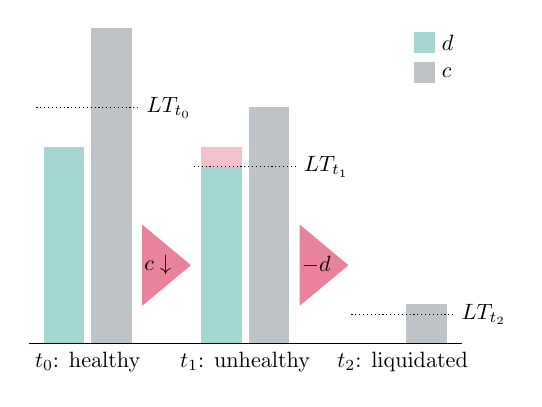
\begin{tikzpicture}[scale=0.5, every node/.style={scale=0.8}]
		
% t0

\filldraw[color = mint] (0.4,0) rectangle ++(1,5);
\filldraw[color = brightanthracite] (1.6,0) rectangle ++(1,8);

\draw [densely dotted, thin] (0.2,6) -- (2.8,6) node [right, text = black]{$LT_{t_0}$};

% t1
\uncover<2-> {
	\draw [softred, fill = softred] (2.9,3) -- (4.1,2) -- (2.9,1) -- (2.9,3) node [midway,right, text = black, xshift = -0.1cm] {$c \downarrow$} -- cycle;

	\filldraw[color = mint] (4.4,0) rectangle ++(1,5);
	\filldraw[softred!50] (4.4,4.5) rectangle ++(1,0.5);
	\filldraw[color = brightanthracite] (5.6,0) rectangle ++(1,6);

	\draw [densely dotted, thin] (4.2,4.5) -- (6.8,4.5) node [right, text = black]{$LT_{t_1}$};
}


% t2

\uncover<3->{
	\draw [softred, fill] (6.9,3) -- (8.1,2) -- (6.9,1) -- (6.9,3) node [midway,right, text = black, xshift = -0.1cm] {$-d$}  -- cycle;

	\filldraw[color = brightanthracite] (9.6,0) rectangle ++(1,1);


	\draw [densely dotted, thin] (8.2,0.75) -- (10.8,0.75) node [right, text = black]{$LT_{t_2}$};
}

% Axis with labels

\draw[-] (0,0) -- (1.5,0) node [below]{$t_0$: healthy} -- (5.5,0) node [below]{$t_1$: unhealthy} -- (9.5,0) node [below]{$t_2$: liquidated} -- (11,0);

\filldraw [mint] (9.8,7.4) rectangle ++ (0.5,0.5);
\node	at (10.3,7.65) [right] {$d$};

\filldraw [brightanthracite] (9.8,6.65) rectangle ++ (0.5,0.5);
\node	at (10.3,6.9) [right] {$c$};
	\end{tikzpicture}
	\caption{Liquidation scenario with $LT = 0.75$}
\end{figure}

	
\end{frame}
%%%	


%%%
\begin{frame}{Liquidations: Two approaches (cont.)}

With protocols unable to become active by themselves, they rely on arbitrageurs to spot and liquidate unhealthy positions.

\vspace{1 em}
Two approaches offering liquidation incentives can be observed: 

\vspace{1 em}
\textbf{1. Discount Sale} (e.g. Aave or Compound)
\vspace{0.2em}
\begin{itemize}
\item Any unhealthy position’s collateral is offered at a discount from the current on-chain oracle price.
\item Liquidator repays (part of the) position’s debt in the respective debt asset and in return receives collateral assets at the discounted price for the repaid amount.
\end{itemize}

\vspace{0.5em}
\textbf{Pro:} Atomic transaction, fast.

\textbf{Con:} Requires high accuracy of on-chain oracle prices at all times.





	
\end{frame}
%%%	


%%%
\begin{frame}{Liquidations: Two approaches }


\textbf{2. Tend \& Dent Auction} (e.g. MakerDAO)
\vspace{0.2em}
\begin{itemize}
\item English auction of an unhealthy position’s collateral can be started by anyone submitting the first bid.
\item Ends when either the maximum auction length is reached or the grace period since the last valid bid.
\item In the \emph{tend phase}, bidders compete by offering to pay larger proportions of the outstanding debt in exchange for the collateral.
\item If there is a bid to pay the debt in full, the auction enters the \textit{dent phase}. Now bidders compete further by accepting a lower proportion of the collateral for repayment of the debt in full.
\end{itemize}
\vspace{0.5em}

\textbf{Pro: }Independent of on-chain oracles.

\textbf{Con: }Time-consuming, costly process for bidders (multiple transactions) and no minimum sale price.


	
\end{frame}
%%%	


%%%
\begin{frame}{Flash Loans Overview}

\begin{minipage}{0.3\textwidth}
	\begin{figure}
		\includegraphics[width=0.7\textwidth]{../assets/images/flashloan}	
	\end{figure}
\end{minipage}
\begin{minipage}{0.65\textwidth}
	Flash loans are a \textbf{concept unique to DeFi}. They are the only loans in the ecosystem that \textbf{do not require collateral}.
\end{minipage}

\uncover<2-> {
\vspace{2em}
In a flash loan, the funds are borrowed, used, and repaid back \textbf{all in one transaction}.
}

\vspace{1em}

\uncover<3-> {
Instead of collateral, lenders rely on \textbf{transaction atomicity}: If principal plus fee is not paid back in the same transaction, all is reverted as if the funds were never granted.
}

\end{frame}
%%%	


%%%
\begin{frame}{Flash Loan Conditions}
For a successful flash loan of $x$ with interest $\rho$  and / or a flat fee $\varphi$:

\vspace{1em}
\begin{enumerate}

\item Unless procured from a CDP, where $x$ can be \textit{flash-minted}, the lending market must \textbf{have $x$ liquid available.}\\
$x \leq LP_{x}$

\item The whole principal plus all interest and fees ($ x(1+\rho) + \varphi$) must be \textbf{returned at the end of the transaction.}

\end{enumerate}

\vspace{1em}
$\Rightarrow$ If conditions are not met, the flash loan transaction is still included in the blockchain but is considered failed, i.e., it does not lead to any state changes except for a nonce update and transaction fee $\epsilon$. 


	
\end{frame}
%%%	


%%%
\begin{frame}{Example of Arbitrage with Flash Loan}

With $x$ as the amount borrowed and sold at the high-price exchange and $x^\ast$ the amount bought back at the low-price exchange with the proceeds, the payoff $\Pi$ can be expressed as:

\begin{equation}
	\Pi = max (x^{\ast}-[x \,(1+\rho) + \varphi ],0) - \epsilon
\end{equation}

\vspace{0.5 em}

\uncover<2->{
\begin{minipage}{0.6\textwidth}
	\begin{figure}[t]
		\centering
		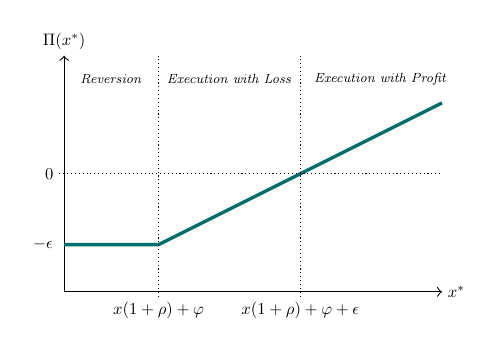
\begin{tikzpicture}[scale=0.6, every node/.style={scale=0.6}]
			
% Axis

\draw[->] (0,0) -- (0,5) node [above ]{$\Pi(x^\ast)$};
\draw[->] (0,0) -- (8,0) node [right] {$x^\ast$};


% Slope

\draw [darkmint, very thick](0,1) node [left, xshift = -0.1cm, black]{$-\epsilon$} -- (2,1) -- (8,4);


% Lines and Labels

\draw [densely dotted, thin] (-0.1,2.5)node [left, black] {$0$} -- (8,2.5);

\draw [densely dotted, thin] (2,-0.1) node [below, black]{$x(1 + \rho) + \varphi$} -- (2,5);

\draw [densely dotted, thin] (5,-0.1) node [below, black]{$x(1 + \rho) + \varphi + \epsilon$} -- (5,5);

\footnotesize

\node at (1,4.5) {\textit{Reversion}};

\node at (3.5,4.5) {\textit{Execution with Loss}};
\node at (6.7,4.5) {\textit{Execution with Profit}};
		\end{tikzpicture}
		\caption{Flash Loan Payoff Diagram}
	\end{figure}
\end{minipage}
\begin{minipage}{0.38 \textwidth}
	Is a corresponding flash loan available when a token pair has a significant price difference on-chain, \textbf{anyone can become an arbitrageur }with the loss potential capped at transaction fee $\epsilon$.
\end{minipage}
}
	
\end{frame}
%%%	


%%%
\begin{frame}{Consequence of Flash Loans}

Flash loans \textbf{effectively remove capital} constraints for any activity that can be performed in one transaction.

\vspace{1em}

\textbf{Common Use Cases}:

\begin{itemize}
\item Collateral swaps (original use case)
\item Arbitrage
\item Portfolio Refactoring
\item Price Manipulation and Wash Trading

\end{itemize}

\vspace{2em}

$\Rightarrow$ While it arguably can be missused, the unique DeFi tool of flash loans have the potential to make markets more efficient and fair.


	
\end{frame}
%%%	


%%%
\begin{frame}{Bib-References}
		Read the Bitcoin Whitepaper, \cite{nakamotoBitcoin2008}.
\end{frame}
%%%

%%%
\begin{frame}%[allowframebreaks]

References must include AAVE, Compund and MAKER Docs
Gervais DeFi Liq Paper, Fabian's Flashloan explainer

\frametitle{References and Recommended Reading}
	\bibliographystyle{amsplain}
	\bibliography{../assets/bib/refs}
\end{frame}
%%%



\end{document}